\chapter{Phương pháp thực nghiệm và kết quả}

Chương này đánh giá ZASSD theo ba khía cạnh: khả năng tái lập phép đo, hiệu năng so với giải mã vanilla và mức độ bảo toàn đầu ra. Các kết quả được chia theo từng cohort. Benchmark paired 150 prompt là nguồn kết quả hiệu năng chính; các phép đo router, phân tích số học và profiling có giao thức riêng nên chỉ được dùng để trả lời câu hỏi tương ứng, không gộp vào trung bình của benchmark chính.

\section{Thiết lập thực nghiệm}

\subsection{Cấu hình benchmark chính}
Bảng~\ref{tab:ch5-main-config} tóm tắt cấu hình ghi trong manifest của benchmark paired. Các phép đo này được thực thi tại commit \texttt{a37a4e4}; revision mô hình, tokenizer, phiên bản thư viện và hash dữ liệu được lưu cùng artifact để có thể kiểm tra lại.

\begin{table}[htbp]
\centering
\small
\caption{Cấu hình của benchmark paired chính}
\label{tab:ch5-main-config}
\begin{tabularx}{\textwidth}{@{}p{3.2cm}X@{}}
\toprule
\textbf{Nhóm} & \textbf{Cấu hình được ghi nhận} \\
\midrule
Phần cứng & NVIDIA GeForce RTX 4050 Laptop GPU; các snapshot nhiệt độ trong phiên chạy dao động 83--88~$^\circ$C. Benchmark chính không lưu thông tin CPU/RAM như một phần của manifest. \\
Hệ điều hành & Linux 6.8.0-94-generic, glibc 2.39; Python 3.12.13. \\
Framework & PyTorch 2.11.0+cu128, CUDA 12.8, Transformers 5.14.1, bitsandbytes 0.50.0. \\
Mô hình & Qwen2.5-3B-Instruct, 36 lớp; model và tokenizer revision \texttt{aa8e72537993ba99e69dfaafa59ed015b17504d1}. \\
Backend & bitsandbytes NF4, tính toán FP16, attention SDPA. \\
Sinh token & Greedy decoding; tối đa 48 token đầu ra; cùng prompt và target model giữa các phương pháp. \\
Mã nguồn & Commit thực thi \texttt{a37a4e4cda647a5f5fc2b6861fb1d28f7db48eea}. \\
\bottomrule
\end{tabularx}
\end{table}

Thông tin phần cứng và phần mềm không hoàn toàn giống nhau giữa mọi thí nghiệm trong repository. Vì vậy, Bảng~\ref{tab:ch5-main-config} chỉ áp dụng cho benchmark chính; những cohort dùng backend, context length hoặc chế độ tracing khác được mô tả riêng tại mục tương ứng.

\section{Tập dữ liệu và giao thức đánh giá}

Benchmark chính gồm 150 prompt: 50 mẫu GSM8K, 50 mẫu HumanEval và 50 mẫu CNN/\allowbreak DailyMail. Mỗi prompt được chạy với giới hạn 48 token sinh. Giao thức gồm hai prompt warmup cho mỗi tập, một repeat và ba seed xoay vòng thứ tự phương pháp (42, 43, 44). Thiết kế này tạo 450 nhóm prompt/thứ tự paired và 2.700 dòng quan sát thô. Mỗi phương pháp được so sánh trên cùng prompt; khi tính khoảng tin cậy, các repeat và seed thứ tự được lấy trung bình trong từng prompt trước khi bootstrap theo prompt.

Thời gian tiền xử lý và sinh được tách thành prefill, thời gian đến khi có logits prompt cuối cùng (TTFT), và decode sau prefill. Trong artifact này, token đầu được chọn từ logits prefill; \texttt{decode\_tokens} không tính token đó, còn end-to-end TPS tính cả prefill. Hai đối chứng kiểm tra overhead cũng được giữ lại: vanilla chạy qua speculative core và PLD bị buộc lookup miss. Cả hai đối chứng giữ nguyên token sequence nhưng chậm hơn direct vanilla, cho thấy có chi phí của đường thực thi/harness; kết quả speedup không được hiệu chỉnh cộng bù overhead này.

\begin{table}[htbp]
\centering
\small
\caption{Các cohort thực nghiệm và phạm vi sử dụng}
\label{tab:ch5-cohorts}
\begin{tabularx}{\textwidth}{@{}p{3.1cm}p{3.3cm}X@{}}
\toprule
\textbf{Cohort} & \textbf{Quy mô/cấu hình} & \textbf{Vai trò trong báo cáo} \\
\midrule
Benchmark paired chính & 150 prompt; NF4; tối đa 48 token & Kết quả throughput, speedup và exact-match của PLD, PLD gate, router; là căn cứ cho kết luận hiệu năng chính. \\
Router paired & 30 prompt; NF4; static KV; tối đa 32 token; K PLD = 2, 4, 8 & Phân tích router trên cohort prompt ngữ cảnh ngắn; có development/held-out, không gộp với benchmark chính. \\
Numerical fidelity & 30 prompt chuẩn bị sẵn; NF4; K=4; tối đa 32 token & So sánh SDPA/eager, static/dynamic và verification tuần tự; thời gian có tracing chỉ mang tính chẩn đoán. \\
Nsight profiling & Một prompt dài 384 token; tối đa 32 token & Quan sát kernel và API trong phiên có instrumentation; không dùng như phép đo production throughput. \\
\bottomrule
\end{tabularx}
\end{table}

\section{Phương pháp đối chứng và chỉ số}

Các phương pháp trong benchmark chính gồm direct vanilla; \textit{vanilla via speculative core} và PLD forced-miss làm đối chứng overhead; PLD với \(K=4\); PLD gate chọn giữa PLD và vanilla; và router chọn giữa PLD \((K\leq4)\), layer-skip \((K=2)\) hoặc vanilla. Do đó, đây là so sánh giữa các phương thức có cùng target model, prompt và cấu hình decode trong một harness, chứ không phải phép đo mọi phương pháp trên mọi backend.

Với prompt \(i\), throughput end-to-end ở một lượt chạy là số token đầu ra chia cho tổng thời gian gồm prefill và decode. Gọi \(r_{m,i,r,o}\) là tỷ số throughput của phương pháp \(m\) với vanilla trên cùng prompt \(i\), cùng repeat \(r\) và seed thứ tự \(o\):

\begin{equation}
r_{m,i,r,o}=\frac{\mathrm{TPS}_{m,i,r,o}}{\mathrm{TPS}_{\mathrm{vanilla},i,r,o}},\qquad
\bar r_{m,i}=\frac{1}{|\mathcal{R}_i|}\sum_{(r,o)\in\mathcal{R}_i}r_{m,i,r,o},\qquad
S_m=\frac{1}{N}\sum_{i=1}^{N}\bar r_{m,i}.
\label{eq:ch5-paired-speedup}
\end{equation}

Do đó, \(S_m\) là trung bình các tỷ số paired ở cấp prompt sau khi gộp các lượt đo của chính prompt đó; nó không phải tỷ số giữa mean TPS của hai phương pháp. CI 95\% được tạo bằng bootstrap prompt: lấy mẫu lại \(N\) prompt có hoàn lại, tính lại \(S_m\) cho mỗi mẫu bootstrap và lấy hai phân vị 2.5\%/97.5\%. Con số PLD \(1.063\times\) trong Bảng~\ref{tab:ch5-main-results} được lấy theo đúng định nghĩa này từ summary/statistics của artifact. Decode TPS là số token decode chia cho thời gian decode và không đồng nhất với end-to-end TPS. Acceptance rate là tỷ lệ draft token được target chấp nhận trên tổng số draft token được đưa ra xác minh. Exact sequence match là tỷ lệ prompt mà toàn bộ token ID đầu ra trùng với direct vanilla. Các chỉ số exactness không suy ra từ acceptance rate.

Peak VRAM trong router evaluation được ghi bằng hàm \path{max_memory_allocated} của PyTorch chia cho \(1024^2\), tức MiB bộ nhớ tensor đã cấp phát cực đại; đây không phải NVML process memory hay bộ nhớ reserved. Tên trường artifact là \texttt{peak\_vram\_mb}, nhưng đơn vị quy đổi thực tế là MiB. Chỉ so sánh trực tiếp trong cùng cohort/cùng phương thức thu thập. Khi báo cáo numerical fidelity, KV drift, logit drift, argmax agreement và sequence identity được xem là các đại lượng riêng: có sai khác tensor không nhất thiết làm đổi token; ngược lại, một token khác làm mất exact sequence match dù phần lớn chuỗi vẫn trùng.

\section{Kết quả benchmark chính}

\subsection{So sánh paired trên ba tập dữ liệu}
Bảng~\ref{tab:ch5-main-results} trình bày kết quả end-to-end speedup từ \path{experiments/benchmark_validation/full_n50_r1_a37a4e4/summary.json}. CI 95\% được bootstrap theo prompt, không coi ba thứ tự chạy của cùng prompt là ba prompt độc lập.

\begin{table}[htbp]
\centering
\small
\caption{Speedup end-to-end và exact sequence match trong benchmark chính}
\label{tab:ch5-main-results}
\begin{tabularx}{\textwidth}{@{}Xrrr@{}}
\toprule
\textbf{Phương pháp} & \textbf{Speedup (95\% CI)} & \textbf{Prompt nhanh hơn vanilla} & \textbf{Exact match} \\
\midrule
Vanilla trực tiếp & 1.000 & -- & 100.0\% \\
Vanilla qua speculative core & 0.970 [0.965, 0.975] & 14.0\% & 100.0\% \\
PLD forced miss & 0.972 [0.968, 0.976] & 13.3\% & 100.0\% \\
PLD, \(K=4\) & \textbf{1.063 [1.036, 1.092]} & 53.3\% & 83.3\% \\
PLD gate & 1.053 [1.025, 1.081] & 48.7\% & 83.3\% \\
Router & 1.050 [1.023, 1.079] & 49.3\% & 83.3\% \\
\bottomrule
\end{tabularx}
\end{table}

PLD đạt speedup trung bình 6.3\% theo tỷ số throughput paired; CI bootstrap không chứa 1 trong cohort này. Tuy nhiên, phân bố theo prompt không đồng đều: median speedup PLD là 1.007, phân vị 10--90 là 0.928--1.258, và 53.3\% prompt nhanh hơn vanilla. Theo từng tập, speedup PLD lần lượt là 1.084 trên GSM8K, 1.115 trên HumanEval và 0.989 trên CNN/DailyMail. Kết quả này cho thấy lợi ích không xuất hiện đồng đều theo workload.

Router đạt 1.050\(\times\) so với vanilla, nhưng tỷ số throughput paired router/PLD là 0.989 (CI 95\%: 0.985--0.993). Như vậy router chậm hơn PLD trong giao thức đã đo, dù vẫn nhanh hơn vanilla ở mức trung bình. PLD gate cũng thấp hơn PLD khoảng 0.9\% theo tỷ số paired. Không nên diễn giải router là cải thiện phương pháp cố định tốt nhất chỉ vì nó có speedup lớn hơn 1 so với vanilla.

\begin{figure}[htbp]
\centering
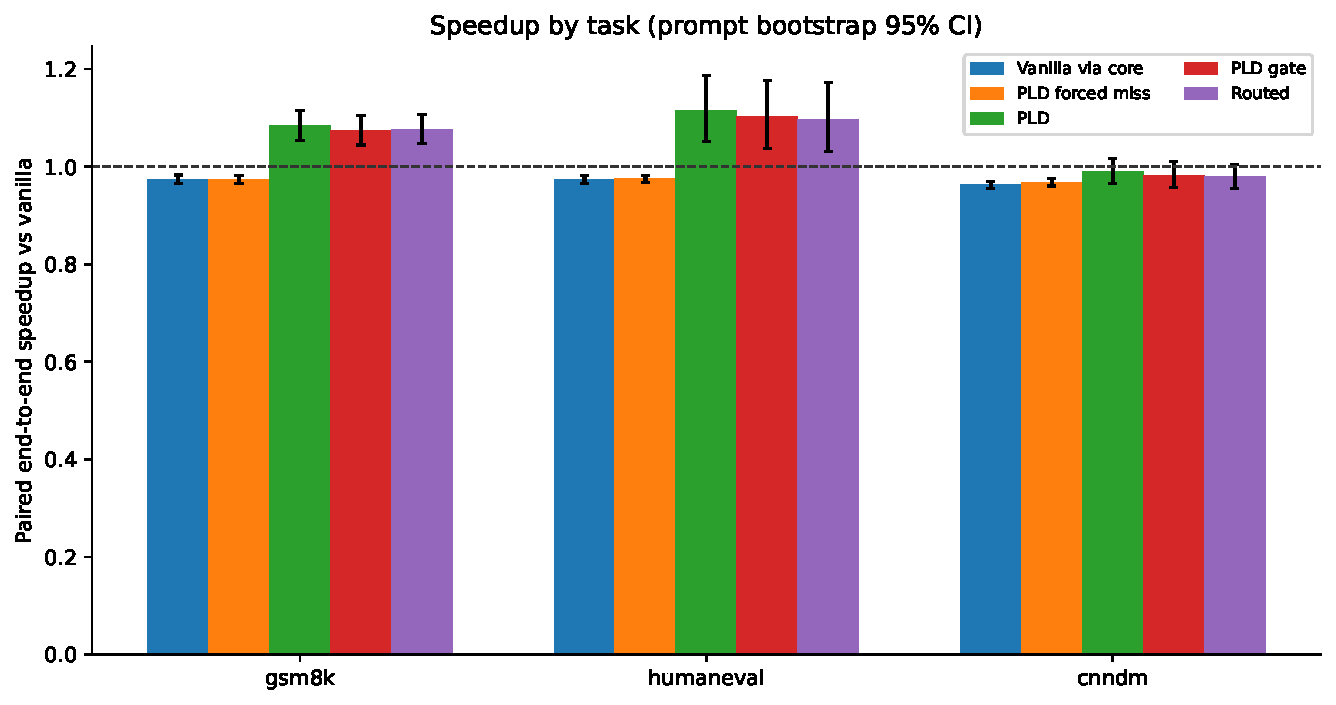
\includegraphics[width=0.88\textwidth]{images/hinh6_speedup_by_task.pdf}
\caption{Speedup end-to-end của các phương pháp theo từng benchmark trong cohort 150 prompt.}
\label{fig:ch5-speedup-task}
\end{figure}

Để làm rõ phân bố ở cấp prompt, Hình~\ref{fig:ch5-paired-distribution} trình bày boxplot speedup paired cho 150 prompt. Trung bình PLD lớn hơn 1 nhưng trung vị chỉ xấp xỉ 1; chỉ 53.3\% prompt nhanh hơn vanilla. Vì vậy, trung bình tổng hợp không có nghĩa PLD cải thiện trên đa số workload với biên độ đồng đều.

\begin{figure}[htbp]
\centering
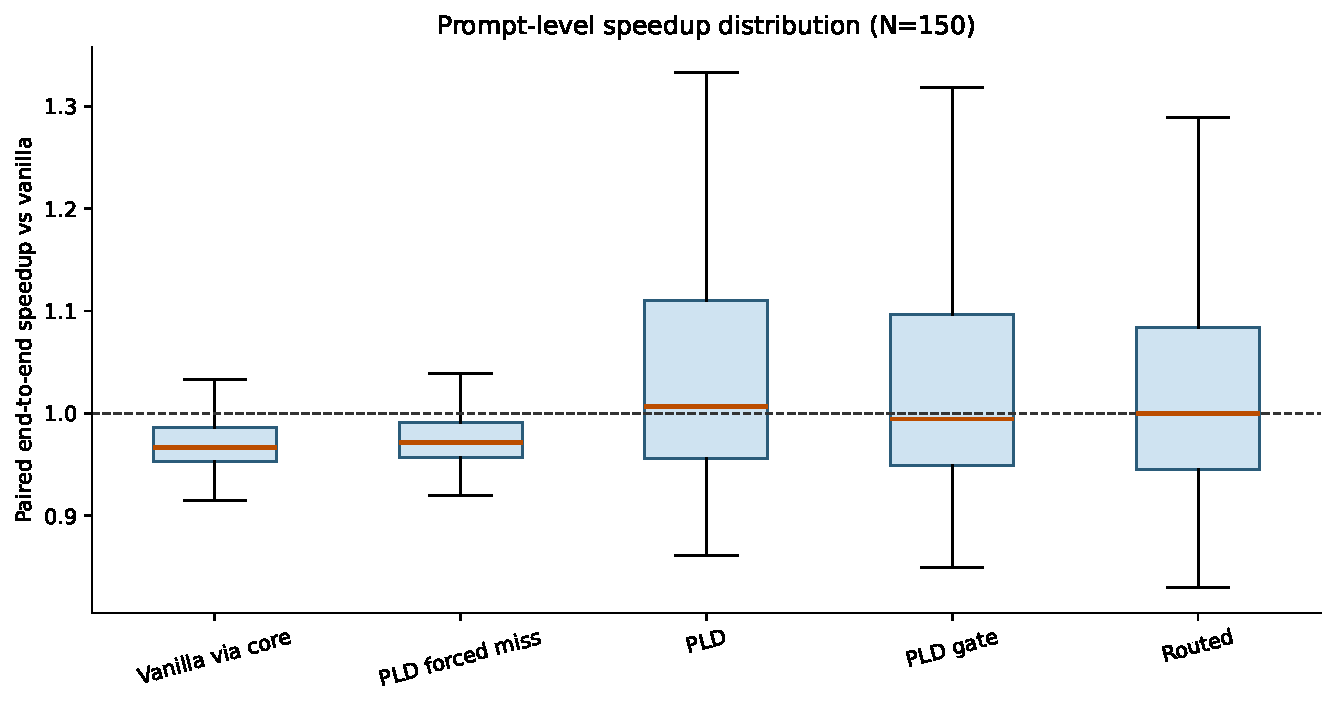
\includegraphics[width=0.88\textwidth]{images/hinh7_paired_speedup.pdf}
\caption{Phân bố speedup end-to-end paired theo prompt; đường đứt đoạn biểu thị hòa vốn \(1.0\times\).}
\label{fig:ch5-paired-distribution}
\end{figure}

Hình~\ref{fig:ch5-speedup-focused} phóng to vùng quanh hòa vốn bằng trục tung thu hẹp từ 0.85 đến 1.20. Các điểm và khoảng tin cậy theo từng tập được vẽ đơn sắc, phân biệt bằng ký hiệu để dễ đọc khi in trắng đen. Khoảng tin cậy là bootstrap theo prompt trong từng tập.

\begin{figure}[htbp]
\centering
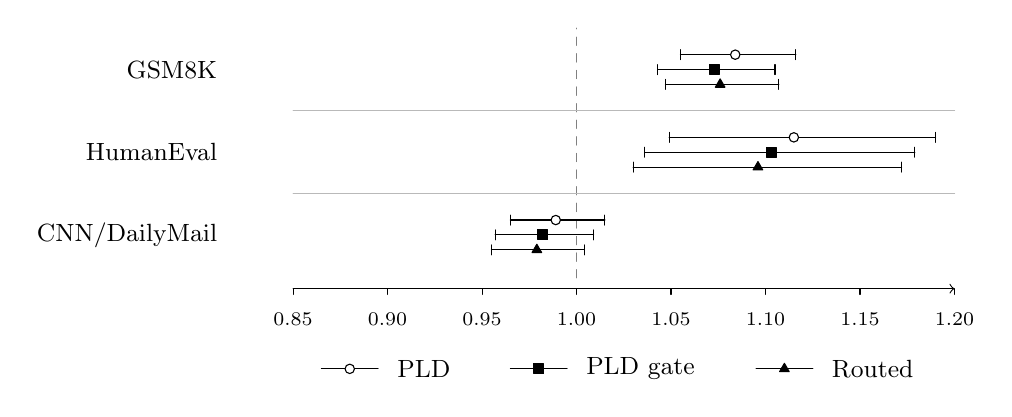
\begin{tikzpicture}[x=24cm,y=1.05cm, line cap=round, line join=round, font=\small]
  % Plot range: x=0 maps to 0.85x; x=0.35 maps to 1.20x.
  \draw[->] (0,0.35) -- (0.35,0.35);
  \foreach \x/\lab in {0/0.85,0.05/0.90,0.10/0.95,0.15/1.00,0.20/1.05,0.25/1.10,0.30/1.15,0.35/1.20} {
    \draw (\x,0.35) -- (\x,0.28) node[below=3pt,font=\scriptsize]{\lab};
  }
  \draw[dashed,gray] (0.15,0.48) -- (0.15,3.5);
  \node[anchor=east] at (-0.035,3) {GSM8K};
  \node[anchor=east] at (-0.035,2) {HumanEval};
  \node[anchor=east] at (-0.035,1) {CNN/DailyMail};
  \draw[gray!55] (0,2.5) -- (0.35,2.5);
  \draw[gray!55] (0,1.5) -- (0.35,1.5);
  % PLD: circle; values are mean ratio and prompt-bootstrap 95\% CI.
  \draw (0.205,3.18)--(0.266,3.18); \draw (0.205,3.12)--(0.205,3.24); \draw (0.266,3.12)--(0.266,3.24); \draw[fill=white] (0.234,3.18) circle (1.7pt);
  \draw (0.199,2.18)--(0.340,2.18); \draw (0.199,2.12)--(0.199,2.24); \draw (0.340,2.12)--(0.340,2.24); \draw[fill=white] (0.265,2.18) circle (1.7pt);
  \draw (0.115,1.18)--(0.165,1.18); \draw (0.115,1.12)--(0.115,1.24); \draw (0.165,1.12)--(0.165,1.24); \draw[fill=white] (0.139,1.18) circle (1.7pt);
  % PLD gate: square.
  \draw (0.193,3.00)--(0.255,3.00); \draw (0.193,2.94)--(0.193,3.06); \draw (0.255,2.94)--(0.255,3.06); \draw plot[mark=square*,mark size=1.8pt] coordinates {(0.223,3.00)};
  \draw (0.186,2.00)--(0.329,2.00); \draw (0.186,1.94)--(0.186,2.06); \draw (0.329,1.94)--(0.329,2.06); \draw plot[mark=square*,mark size=1.8pt] coordinates {(0.253,2.00)};
  \draw (0.107,1.00)--(0.159,1.00); \draw (0.107,0.94)--(0.107,1.06); \draw (0.159,0.94)--(0.159,1.06); \draw plot[mark=square*,mark size=1.8pt] coordinates {(0.132,1.00)};
  % Routed: triangle.
  \draw (0.197,2.82)--(0.257,2.82); \draw (0.197,2.76)--(0.197,2.88); \draw (0.257,2.76)--(0.257,2.88); \draw plot[mark=triangle*,mark size=2pt] coordinates {(0.226,2.82)};
  \draw (0.180,1.82)--(0.322,1.82); \draw (0.180,1.76)--(0.180,1.88); \draw (0.322,1.76)--(0.322,1.88); \draw plot[mark=triangle*,mark size=2pt] coordinates {(0.246,1.82)};
  \draw (0.105,0.82)--(0.154,0.82); \draw (0.105,0.76)--(0.105,0.88); \draw (0.154,0.76)--(0.154,0.88); \draw plot[mark=triangle*,mark size=2pt] coordinates {(0.129,0.82)};
  % Monochrome legend.
  \draw (0.015,-0.62)--(0.045,-0.62); \draw[fill=white] (0.030,-0.62) circle (1.7pt); \node[anchor=west] at (0.05,-0.62) {PLD};
  \draw (0.115,-0.62)--(0.145,-0.62); \draw plot[mark=square*,mark size=1.8pt] coordinates {(0.130,-0.62)}; \node[anchor=west] at (0.15,-0.62) {PLD gate};
  \draw (0.245,-0.62)--(0.275,-0.62); \draw plot[mark=triangle*,mark size=2pt] coordinates {(0.260,-0.62)}; \node[anchor=west] at (0.28,-0.62) {Routed};
\end{tikzpicture}
\caption{Speedup theo tập trên vùng tập trung 0.85--1.20\(\times\); trục tung được thu hẹp để thấy rõ chênh lệch quanh đường hòa vốn 1.0\(\times\). Ký hiệu đơn sắc: hình tròn PLD, hình vuông PLD gate, tam giác router; thanh ngang là CI bootstrap 95\%.}
\label{fig:ch5-speedup-focused}
\end{figure}

Các negative control vanilla-via-core và PLD-forced-miss chậm hơn vanilla trực tiếp lần lượt khoảng 3.0\% và 2.8\%. Đây là overhead quan sát được của đường thực thi trong harness, không phải một hiệu chỉnh để cộng vào kết quả PLD. Việc giữ control giúp phân biệt lợi ích do lookup trúng với chi phí nền của speculative path.

\subsection{Layer-skip và router trên cohort riêng}
Trong đánh giá router độc lập gồm 30 prompt ngữ cảnh 384 token, CKA90 với \(K=2\) đạt 0.902\(\times\) vanilla (CI 95\%: 0.875--0.929), trong khi hybrid router đạt 1.045\(\times\) (1.001--1.090) và PLD \(K=2\) được chọn từ development đạt 1.095\(\times\) (1.054--1.139). Trên 14 prompt held-out, CKA90 đạt 0.917\(\times\) (0.880--0.956), router 1.078\(\times\) (1.022--1.142), PLD \(K=2\) 1.134\(\times\) (1.081--1.194). Đây là cohort prepared-input ngắn, một lượt mỗi prompt; nó cho thấy cấu hình layer-skip được khảo sát chậm hơn vanilla, nhưng không thể dùng để kết luận mọi cách chọn lớp hoặc mọi context đều chậm.

\section{Phân tích chi phí và điều kiện hòa vốn}

Speculative decoding chỉ có lợi khi thời gian hoàn thành một cycle đủ thấp so với số token thực sự được phát ra trong cycle đó. Với thời gian vanilla trung bình mỗi token \(T_v\), điều kiện hòa vốn có thể viết \(\mathbb{E}[T_{\mathrm{cycle}}] < \mathbb{E}[N_{\mathrm{emit}}]T_v\). Vì vậy acceptance cao tự nó không chứng minh tăng throughput: một draft tốn thời gian hoặc target verification đắt có thể xóa hết lợi ích của nhiều token được chấp nhận. Mô hình ở Chương~3 được dùng như quan hệ giải thích; phép đo phải tránh cộng chồng các khoảng thời gian đồng thời.

\begin{equation}
T_{\mathrm{cycle}} = T_{\mathrm{draft}} + T_{\mathrm{verify}} + T_{\mathrm{cache}} + T_{\mathrm{lookup}} + T_{\mathrm{control}} + T_{\mathrm{sync}},
\label{eq:ch5-cycle-cost}
\end{equation}

Trong đó các thành phần chỉ được cộng trực tiếp khi được đo trên các khoảng không chồng lấn; các tổng thời gian API host và kernel GPU của profiler không thể cộng cơ học với nhau. Tại benchmark chính, PLD có speedup nhưng router và PLD gate thấp hơn PLD; điều này phù hợp với việc quyết định/fallback bổ sung có chi phí, song benchmark tổng thể không đủ để quy toàn bộ chênh lệch cho riêng một thành phần.

Artifact benchmark lưu số token decode, tổng số verification cycle, số cycle PLD/layer-skip, accepted tokens và tổng decode wall time. Từ các bộ đếm này có thể suy ra một số thống kê gộp như Bảng~\ref{tab:ch5-cycle-stats}. Các giá trị là tỷ số tổng trên 450 lượt prompt/order của mỗi phương pháp, không phải trung bình không trọng số của từng cycle.

Đây là thống kê mô tả gộp được suy ra từ bộ đếm tổng; artifact không lưu thời gian độc lập cho từng cycle. Vì vậy, các giá trị này giúp kiểm tra quan hệ tổng thể giữa số token, số cycle và thời gian, nhưng không xác định chi phí thành phần hay nguyên nhân thời gian của từng cycle.

\begin{table}[htbp]
\centering
\small
\caption{Thống kê cycle gộp suy ra từ raw benchmark paired}
\label{tab:ch5-cycle-stats}
\begin{tabularx}{\textwidth}{@{}>{\centering\arraybackslash}p{2.4cm}>{\centering\arraybackslash}p{2.8cm}>{\centering\arraybackslash}p{3.0cm}>{\centering\arraybackslash}p{2.8cm}>{\centering\arraybackslash}p{2.6cm}@{}}
\toprule
\textbf{Phương pháp} & \textbf{\shortstack{Accepted tokens\\per spec cycle}} & \textbf{\shortstack{Decode tokens\\per verify cycle}} & \textbf{\shortstack{Decode time\\per cycle (ms)}} & \textbf{\shortstack{Vanilla fallback\\cycles}} \\
\midrule
PLD \(K=4\) & 1.134 & 1.217 & 31.82 & 78.5\% \\
Router & 1.125 & 1.227 & 32.51 & 77.5\% \\
\bottomrule
\end{tabularx}
\end{table}

Số candidate draft được đề xuất mỗi cycle không được lưu trong raw file, nên không thể tính trực tiếp đại lượng này hoặc acceptance fraction trên tổng candidates từ artifact hiện tại. Số cycle không draft là phần dư giữa tổng verification cycles và số PLD/layer-skip cycles, dựa trên các trường đếm của harness; vì vậy được xem là thống kê suy ra. Thời gian mỗi cycle được tính bằng tổng decode wall time chia tổng verification cycles. Với vanilla baseline, decode wall time gộp tương ứng khoảng 27.19~ms/token. Thay các thống kê gộp vào \(\mathbb{E}[N_{\mathrm{emit}}]T_v/\mathbb{E}[T_{\mathrm{cycle}}]\) cho decode-only ratio khoảng 1.041 cho PLD và 1.026 cho router; các tỷ số này khớp với pooled decode TPS tính từ cùng token/time totals theo định nghĩa, nên là kiểm tra nhất quán số học chứ không phải dự đoán độc lập. Chúng cũng không thay thế end-to-end paired speedup ở mục~5.4 vì công thức này không tính prefill.

Để khảo sát chi phí ở mức kernel, một phép Nsight riêng chạy trên cùng một prompt 384 token, NF4/FP16, SDPA và giới hạn 32 token. Bảng~\ref{tab:ch5-nsys} tổng hợp thời gian kernel GPU (tổng các kernel có thể chồng lấn) và tổng thời gian API host cho đồng bộ/phát lệnh. Đây là số liệu có instrumentation, không phải end-to-end latency production.

\begin{table}[htbp]
\centering
\small
\caption{Một số số đo Nsight chẩn đoán trên một prompt cố định}
\label{tab:ch5-nsys}
\begin{tabularx}{\textwidth}{@{}Xrrrr@{}}
\toprule
\textbf{Phương pháp} & \textbf{Tổng GPU kernel (ms)} & \textbf{NF4 GEMM (ms)} & \textbf{Dequant (ms)} & \textbf{Sync API (ms)} \\
\midrule
Vanilla & 828.2 & 312.8 & 66.5 & 378.1 \\
PLD \(K=4\) & 811.1 & 400.0 & 54.3 & 270.6 \\
CKA90 \(K=2\) & 951.7 & 451.7 & 40.0 & 376.8 \\
\bottomrule
\end{tabularx}
\end{table}

Số liệu cho thấy thành phần NF4 GEMM, dequant và các lời gọi đồng bộ đều hiện diện đáng kể trong trace. Tuy nhiên, tổng GPU kernel có thể bao gồm overlap, còn synchronize API là thời gian host-side; chúng không phải các thành phần độc lập của critical path. Do đó, từ trace này chỉ có thể mô tả hoạt động quan sát được, chưa thể kết luận dequant hoặc synchronization là nguyên nhân duy nhất gây chậm. Manifest và các tệp xuất Nsight được lưu tại \path{experiments/backend_validation/kernel_profile/}.

\section{Đánh giá bộ nhớ và tính đúng đắn}

\subsection{Bộ nhớ}
Các phương pháp khảo sát không nạp thêm checkpoint draft, nhưng điều đó không đồng nghĩa với không phát sinh thêm VRAM: vẫn có KV cache, activation, vùng làm việc kernel và buffer đã cấp phát. Trong router evaluation 30 prompt (một cohort khác benchmark chính), peak allocated memory trung bình ghi nhận khoảng 2\,107~MiB cho direct vanilla, 2\,110~MiB cho PLD \(K=2\), 2\,111~MiB cho PLD \(K=4\), 2\,112~MiB cho CKA90 \(K=2\), và 2\,113~MiB cho hybrid router. Đây là giá trị trung bình của \texttt{torch.cuda.max\_memory\_allocated}, không phải VRAM NVML/reserved. Chênh lệch nhỏ trong phép đo này không thể khái quát sang mọi context length, backend hoặc cơ chế cấp phát; đây cũng không phải số liệu peak VRAM của cohort 150 prompt.

\subsection{Numerical fidelity và sequence identity}
Benchmark paired chính có exact sequence match 83.3\% cho PLD, PLD gate và router. Phân tích can thiệp trên chính nhóm 25 prompt mismatch (7 GSM8K, 5 HumanEval, 13 CNN/DailyMail) ghi nhận vanilla lặp lại ổn định; trace mặc định có khác biệt digest active KV trước token mismatch, còn verification tuần tự canonical khớp vanilla đủ 48 token trên các prompt này. Kết quả là bằng chứng mạnh cho sự phụ thuộc đường tính toán/cache trong cấu hình NF4 đã thử, nhưng không chứng minh cùng tỷ lệ divergence ở precision hoặc backend khác.

Một kiểm chứng riêng trên 30 prompt, giới hạn 32 token và \(K=4\), phân chia 16 prompt chẩn đoán và 14 held-out cho thấy ảnh hưởng của backend/chế độ thực thi. Mười sáu ID chẩn đoán được lấy từ cohort PLD \(K=4\) ngữ cảnh ngắn đã ghi nhận mismatch trong phép chạy độc lập trước đó; chúng được chọn để khảo sát nguyên nhân sai khác, không lấy ngẫu nhiên từ traffic. Mười bốn ID held-out là các mẫu còn lại trong cùng prepared-input artifact và không được dùng khi chọn nhóm chẩn đoán, nhưng cũng không phải một tập dữ liệu ngoài độc lập. Bảng~\ref{tab:ch5-fidelity} báo cáo sequence match và các chỉ số drift tách biệt.

\begin{table}[htbp]
\centering
\small
\caption{Kết quả numerical fidelity trên cohort 30 prompt; thời gian có tracing chỉ mang tính chẩn đoán}
\label{tab:ch5-fidelity}
\begin{tabularx}{\textwidth}{@{}Xlrrr@{}}
\toprule
\textbf{Cấu hình} & \textbf{Cohort} & \textbf{Exact match} & \textbf{KV/logit drift} & \textbf{Token divergence} \\
\midrule
SDPA, static, batched & Diagnostic (16) & 0/16 & 16/16 & 16/16 \\
SDPA, static, batched & Held-out (14) & 14/14 & 14/14 & 0/14 \\
Eager, static, batched & Diagnostic (16) & 8/16 & 16/16 & 8/16 \\
Eager, static, batched & Held-out (14) & 14/14 & 14/14 & 0/14 \\
SDPA, dynamic, batched & Diagnostic (16) & 0/16 & 16/16 & 16/16 \\
SDPA, dynamic, batched & Held-out (14) & 14/14 & 14/14 & 0/14 \\
SDPA, static, tuần tự & Diagnostic (16) & 16/16 & 0/16 & 0/16 \\
SDPA, static, tuần tự & Held-out (14) & 14/14 & 0/14 & 0/14 \\
\bottomrule
\end{tabularx}
\end{table}

Trong các hàng batched held-out, drift KV/logit được ghi nhận nhưng token sequence vẫn trùng vanilla; đây là ví dụ trực tiếp cho thấy numerical equivalence và sequence identity không tương đương. Mức 0/16 exact match của SDPA batched trên nhóm chẩn đoán là kết quả có điều kiện trên một cohort được chọn vì từng có mismatch, không phải ước lượng tỷ lệ lỗi cho workload tự nhiên. Tương ứng, 14/14 exact match held-out chỉ mô tả 14 mẫu chưa chọn trong cùng artifact; cỡ mẫu nhỏ và nguồn mẫu chung không cho phép kết luận xác suất lỗi thực tế bằng 0. Ở nhóm chẩn đoán, chuyển sang verification tuần tự khôi phục exact match 16/16, đồng thời làm TPS chẩn đoán giảm so với cấu hình batched. Các con số thời gian tại đây có tracing snapshot overhead nên không được so với benchmark production ở mục~5.4.

\subsection{Kiểm tra logic KV cache}
Các test về prefix không bị draft ghi đè, target verification và rollback được mô tả tại Chương~4 và nằm trong \path{tests/test_kv_cache_invariants.py}. Chúng kiểm tra invariant ở mức cấu trúc cache/logical length, trong khi cohort numerical fidelity ở trên đánh giá sai khác tensor và token trên các prompt cụ thể. Hai nhóm bằng chứng bổ sung cho nhau: test invariant không tự bảo đảm logits hoặc chuỗi token luôn tương đương vanilla. Kết quả kiểm thử chỉ nên gắn với log chạy tương ứng; không suy rộng sang các cấu hình chưa chạy.

\section{Thảo luận và giới hạn}

Bảng~\ref{tab:ch5-rq} tóm tắt câu trả lời thực nghiệm trong phạm vi các cohort hiện có.

\begin{table}[htbp]
\centering
\small
\caption{Tổng hợp kết quả theo câu hỏi nghiên cứu}
\label{tab:ch5-rq}
\begin{tabularx}{\textwidth}{@{}p{1.3cm}X@{}}
\toprule
\textbf{Câu hỏi} & \textbf{Kết luận có giới hạn theo bằng chứng} \\
\midrule
RQ1 & PLD tăng tốc trung bình trên cohort 150 prompt (1.063\(\times\)), nhưng hiệu quả phụ thuộc tập dữ liệu; CNN/DailyMail đạt 0.989\(\times\). CKA90/K2 chậm hơn vanilla trong cohort router 30 prompt đã thử. \\
RQ2 & Draft, verify, lookup, điều khiển và đồng bộ cùng ảnh hưởng thời gian cycle. Nsight cho thấy các hoạt động GEMM, dequant và sync, nhưng phép profiling đơn lẻ chưa xác định critical path nhân quả. Acceptance cao không bảo đảm tăng tốc. \\
RQ3 & Với NF4, batched execution có các trường hợp KV/logit drift và token divergence; verification tuần tự khớp vanilla trên cohort fidelity đã thử nhưng chậm hơn trong phép đo có tracing. Kết luận không thay thế kiểm chứng trên precision/backend khác. \\
RQ4 & Router tăng tốc so với vanilla trong benchmark chính (1.050\(\times\)) nhưng thấp hơn PLD (tỷ số paired 0.989; CI 0.985--0.993). Router hiện chưa chứng minh lợi ích so với fixed PLD trong giao thức này. \\
\bottomrule
\end{tabularx}
\end{table}
Các giới hạn chính gồm: benchmark hiệu năng chính chạy trên một GPU và một cấu hình NF4/SDPA; tốc độ biến thiên theo prompt và tập dữ liệu; exact sequence match thấp hơn 100\% trong phương pháp suy đoán; các phép router, fidelity và profiling dùng cohort/cấu hình riêng; profiling có instrumentation; và chưa có cơ sở để khái quát sang mô hình, GPU, precision hay backend khác. Các thí nghiệm context/backend exploratory cũng không được trộn vào kết quả xác nhận của benchmark 150 prompt.

Trong điều kiện GPU VRAM hạn chế, một kỹ thuật speculative decoding đáng sử dụng khi đồng thời thỏa ba điều kiện có thể kiểm chứng: (1) tổng chi phí cycle đủ thấp so với số token được phát ra, thay vì chỉ có acceptance cao; (2) nó cải thiện trên baseline cố định mạnh nhất đã đo, không chỉ vượt vanilla; và (3) mức speedup đáp ứng yêu cầu numerical fidelity/sequence identity của ứng dụng. Trong thí nghiệm này, PLD vượt vanilla trung bình nhưng có mismatch token và không nhanh hơn trên CNN/DailyMail; router vẫn dưới PLD; verification tuần tự khôi phục sequence identity trong cohort fidelity nhưng tốn thời gian hơn. Vì vậy, lựa chọn thực tế phụ thuộc vào workload, ngân sách latency và yêu cầu chính xác đầu ra.
